% =====================================================================
% Section IV: Experiments.  \input{} from main.tex inside \section{Experiments}.
% Every number here is traceable to a run in configs/run_plan.yaml; cost figures
% come from the single-session M1-v3 benchmark.
% =====================================================================

\subsection{Experimental Setup}
\label{sec:setup}

\textbf{Datasets.} We evaluate on Tiny-ImageNet \cite{tinyimagenet} (200
classes) and CIFAR-10 \cite{cifar} (10 classes). Both are processed at $32\times32$
resolution. For Tiny-ImageNet this means downsampling from the native
$64\times64$, which discards information and makes our absolute numbers
\emph{not} comparable to work that evaluates at $64\times64$; we adopt it
deliberately, because the regime this paper studies is low-resolution
classification under a tight parameter budget, and we hold it fixed across
every model so that all comparisons reported here are internally valid.
Tiny-ImageNet does not release labels for its test split, so we use the
official 10{,}000-image validation split as our \emph{test} set and hold out
a further 10{,}000 images from the training split, drawn with a fixed seed,
as the validation set used for model selection. No model ever selects an
epoch using the reported test set.

\textbf{Budget parity.} Every model, proposed or baseline, is trained for the
same number of epochs on a given dataset: 100 on Tiny-ImageNet and 250 on
CIFAR-10. We use identical augmentation --- RandAugment \cite{randaugment},
random erasing \cite{randomerasing}, mixup \cite{mixup} and CutMix
\cite{cutmix} --- the same optimiser and schedule, and the same batch size. No
model receives a tuned recipe of its own.

\textbf{Knowledge distillation.} Where distillation is used, every student,
\emph{including every baseline}, is distilled from a ResNet-18 teacher
\cite{resnet} trained on the same dataset and the same seed, with the same
loss: $\alpha = 0.5$ and temperature $T = 4$ \cite{hinton}. We report both
cross-entropy (CE) and distilled (KD) results for all models, so that no
comparison mixes training signals.

\textbf{Seeds and statistics.} Headline configurations are trained with three
seeds ($42, 43, 44$); tables report the mean and standard deviation, with the
number of runs $n$ given explicitly. Differences between groups are tested
two ways. At the seed level we use Welch's unequal-variance $t$-test on the
three per-seed accuracies. Within a seed we use an exact paired McNemar test
\cite{mcnemar} on the $10{,}000$ test predictions of the two models being
compared, which uses the pairing that a $t$-test over seed means discards. We report both
because they answer different questions, and we state $n$ wherever it is
below three.

\textbf{Counting operations.} Multiply--accumulate counts for the clustering
branch are easy to understate, and the first version of this work did. An
automatic counter sees the similarity matrix as a matrix product and counts
it, but the aggregation and dispatch steps are element-wise multiplications
followed by reductions, which most counters skip. For $N$ points, $M$ centres
per fold tile and head dimension $d$, each of the three steps costs $NMd$ per
head, so a counter that sees only the first reports a third of the branch's
arithmetic. We instrument the clustering operation directly and add the two
uncounted terms, which is why the operation counts we report for clustering
models are higher than a naive profile would give. For the proposed model the
correction is zero, since it contains no clustering.

\textbf{Reproducibility.} Every run writes a provenance record containing the
git commit, the seed, the resolved teacher checkpoint and the full software
and hardware environment, together with its per-image test predictions. The
code, the configuration of every run reported here, and those per-run records
are available at \url{https://github.com/nvhungus/context-cluster-ablation}.

% ---------------------------------------------------------------------
\subsection{Main Results}
\label{sec:main}

Table~\ref{tab:main} reports both datasets. Under distillation the proposed
All-Local model reaches $61.21 \pm 0.40$ top-1 on Tiny-ImageNet, against $59.72 \pm 0.14$ for
the parameter-matched ShuffleNetV2-x1.5 \cite{shufflenetv2} trained
identically from the same teacher. The margin of $+1.49$ pp is significant at
the seed level (Welch $t = 6.10$, $p = 0.016$) and, independently, on each of
the three seeds under a paired McNemar test. The same model exceeds the
ResNet-18 teacher that supervised it by $+2.46$ pp ($p = 0.008$) while using
$4.16\times$ fewer parameters and $2.41\times$ fewer multiply--accumulate
operations. The comparison holds on CIFAR-10, where
the proposed model leads ShuffleNetV2-x1.5 by $+0.82$ pp with distillation
(McNemar $p = 0.009$) and by $+0.64$ pp without it ($p = 0.014$), and is
statistically indistinguishable from the teacher ($-0.08$ pp validation,
$+0.15$ pp test, $p = 0.432$) at $4.25\times$ fewer parameters.

\textbf{The cross-entropy picture is weaker, and we state it plainly.}
Without distillation the proposed model reaches $58.69 \pm 0.10$ against
$58.22 \pm 0.23$ for ShuffleNetV2-x1.5. That $+0.47$ pp margin does not reach
significance at the seed level ($p = 0.051$), and against the ResNet-18
teacher the proposed model is $-0.07$ pp, a tie ($p = 0.405$). The
beat-the-teacher result reported above therefore holds \emph{in the distilled
setting}, and we condition every such claim on that setting rather than
presenting it as an unconditional property of the architecture.

\textbf{An asymmetry we observe but do not explain.} Given the identical
distillation recipe, the proposed model gains $+2.52$ pp from distillation
while ShuffleNetV2-x1.5 gains $+1.50$ pp and ShuffleNetV2-x1.0 gains $+1.58$
pp. The proposed design converts the same teacher signal into roughly one
additional percentage point. We note that this is not explained by headroom:
the proposed model has the \emph{higher} cross-entropy accuracy of the pair
and therefore less room to improve, yet gains more. We have not tested a
mechanism for this and do not propose one; we report it as an observation and
leave it to future work. What the comparison does establish is that under a
fixed, identical distillation protocol applied to every model, the proposed
architecture is the more accurate one at a matched parameter budget.

\textbf{A caveat about the MobileNetV2 row.} MobileNetV2 is the clear outlier
in Table~\ref{tab:main}: at 2.48M parameters it reaches $49.25$ on
Tiny-ImageNet, $6.53$ pp below a ShuffleNetV2-x1.0 that carries $41\%$ fewer
parameters. The cause is resolution, and part of it is our own adaptation.
Each of these networks was designed for $224\times224$ and reduces resolution
$32\times$ end to end, which leaves a $1\times1$ map at $32\times32$ input, so
all of them need their downsampling schedule shortened. For ResNet-18 and both
ShuffleNetV2 widths we removed two reduction steps, setting the stem to
stride~1 and replacing the max-pool with an identity, which leaves a
$4\times4$ final feature map. MobileNetV2 has no max-pool to remove, and we
changed only its stem stride; its four stride-2 inverted-residual stages
survive untouched, so it still reduces resolution $16\times$ and finishes on a
$2\times2$ map. Its operation count is the symptom: 25.8M MACs, the lowest in
the table and $1.8\times$ below ShuffleNetV2-x1.0 despite $70\%$ more
parameters. Most of its capacity sits in channels it can no longer resolve
spatially.

We report this because it means MobileNetV2 is a weaker baseline here than a
more carefully adapted version would be, and the weakness flatters our
results. It is also the reason we treat ShuffleNetV2-x1.5 rather than
MobileNetV2 as the primary comparison throughout. Read charitably, the row is
a second and independent instance of the effect that dominates
Section~\ref{sec:ablation}: at $32\times32$ the decisive variable is how early
a network discards spatial resolution, and a design that discards it twice
over cannot be rescued by parameters.

% Merged into one full-width float: the five-column single-column version
% overflowed \columnwidth and collided with the CIFAR-10 table. Keeping both
% datasets in one table* also removes the float-ordering hazard that arises
% when a table* and a table are queued separately.
\begin{table*}[!t]
\renewcommand{\arraystretch}{1.15}
\caption{\uppercase{Main results. Top-1 accuracy (\%) at $32\times32$, mean $\pm$ standard
deviation over $n$ seeds. Tiny-ImageNet: 100 epochs, $n$ as shown. CIFAR-10:
250 epochs, single seed. Every distilled student uses the same ResNet-18
teacher trained on the same dataset and seed, with $\alpha = 0.5$ and $T = 4$.
ResNet-18 is that teacher, so it is trained with cross-entropy only and has no
KD entry. Parameters and MACs are for the 200-class head; the CIFAR-10
variants differ only in the classifier.}}
\label{tab:main}
\centering
\footnotesize
\begin{tabular}{@{}lrrcccc@{}}
\toprule
& & & \multicolumn{2}{c}{Tiny-ImageNet} & \multicolumn{2}{c}{CIFAR-10} \\
\cmidrule(lr){4-5}\cmidrule(lr){6-7}
Model & Params & MACs & CE ($n$) & KD ($n$) & CE & KD \\
\midrule
ResNet-18 (teacher) \cite{resnet} & 11.27M & 556.8M & $58.76${\scriptsize$\pm$0.06} (3) & -- & $96.76$ & -- \\
MobileNetV2 \cite{mobilenetv2} & 2.48M & 25.8M & $49.25$ (1) & $52.32$ (1) & $94.06$ & $94.28$ \\
ShuffleNetV2-x1.0 \cite{shufflenetv2} & 1.46M & 46.3M & $55.78${\scriptsize$\pm$0.30} (3) & $57.36${\scriptsize$\pm$0.40} (3) & $95.40$ & $95.22$ \\
ShuffleNetV2-x1.5 \cite{shufflenetv2} & 2.68M & 96.1M & $58.22${\scriptsize$\pm$0.23} (3) & $59.72${\scriptsize$\pm$0.14} (3) & $95.56$ & $95.86$ \\
Context Cluster \cite{coc} & 2.46M & 34.4M & $49.45$ (1) & -- & $92.74$ & -- \\
Hybrid baseline ($\rho{=}0.5$) & 1.80M & 138.9M & $56.40${\scriptsize$\pm$0.21} (3) & $58.19${\scriptsize$\pm$0.25} (3) & $95.44$ & $96.16$ \\
\midrule
\textbf{All-Local (ours)} & 2.71M & 231.3M & $\mathbf{58.69}${\scriptsize$\pm$0.10} (3) & $\mathbf{61.21}${\scriptsize$\pm$0.40} (3) & $\mathbf{96.20}$ & $\mathbf{96.68}$ \\
\bottomrule
\end{tabular}
\end{table*}

% ---------------------------------------------------------------------
\subsection{Ablation Study}
\label{sec:ablation}

Table~\ref{tab:ablation} varies one design decision at a time from the hybrid
model, holding the stem, fold partitioning, block depth and width fixed so
that each row isolates a single factor.

\textbf{Clustering does not pay for itself.} Setting $\rho = 0$, which removes
the local convolutional branch and leaves pure clustering while keeping every
other choice identical, costs $0.74$ pp. Setting $\rho = 1$ instead, removing
the clustering branch entirely, \emph{gains} $+1.03$ pp while using 10\% fewer
parameters. The two rows bracket the question the paper asks: at this scale and
resolution the local branch is what carries the accuracy, and the clustering
branch is a net cost.

\textbf{The supporting design choices contribute little.} Removing fold
partitioning ($+0.20$ pp) and removing channel shuffle ($+0.25$ pp) both leave
accuracy unchanged within run-to-run variation, so neither is load-bearing.
Changing cluster occupancy in either direction hurts, by $1.02$ pp at $r = 1$
and $0.80$ pp at $r = 4$, and giving stage~4 four centres instead of one costs
$0.31$ pp. The single largest effect in the table is the stem stride: moving
from stride~1 to stride~2 costs $5.72$ pp. Because that change halves the
resolution entering every stage as well as altering cluster occupancy, we
attribute the bulk of it to resolution rather than to clustering.

\textbf{The hand-designed local operator is replaceable.}
Table~\ref{tab:operator} compares the fixed sparse LBP-pattern filters used at
stage~1 of the hybrid model against a plain learned $3\times3$ convolution at
matched parameters. At 1.62M parameters the learned convolution is ahead by
$0.10$ pp (McNemar $p = 0.63$); at the 2.71M scale of the proposed model the
two are indistinguishable over three seeds ($61.21 \pm 0.40$ against
$61.23 \pm 0.28$, Welch $p = 0.956$). The learned convolution nevertheless
uses $2.50\times$ less peak activation memory at batch 128, because the fixed
filters expand the channel count eightfold before projecting back. We
therefore adopt the learned convolution: the hand-designed operator buys no
accuracy and costs memory.

\begin{table}[!t]
\renewcommand{\arraystretch}{1.15}
\caption{\uppercase{One-change ablations on Tiny-ImageNet, cross-entropy.
Each row changes exactly one design decision from the hybrid baseline.}}
\label{tab:ablation}
\centering
\footnotesize
\begin{tabular}{@{}lccr@{}}
\toprule
Configuration & Top-1 (\%) & $n$ & $\Delta$ \\
\midrule
Hybrid baseline ($\rho{=}0.5$) & $56.40${\scriptsize$\pm$0.21} & 3 & -- \\
\midrule
$\rho = 0$ (clustering only) & $55.66${\scriptsize$\pm$0.20} & 3 & $-0.74$ \\
$\rho = 1$ (local only, 1.62M) & $57.43${\scriptsize$\pm$0.14} & 3 & $\mathbf{+1.03}$ \\
\midrule
No fold partitioning & $56.60$ & 1 & $+0.20$ \\
No channel shuffle & $56.65$ & 1 & $+0.25$ \\
Stage-4 $2\times2$ proposals & $56.09$ & 1 & $-0.31$ \\
Occupancy $r = 1$ & $55.38$ & 1 & $-1.02$ \\
Occupancy $r = 4$ & $55.60$ & 1 & $-0.80$ \\
Stem stride $1 \rightarrow 2$ & $50.68$ & 1 & $\mathbf{-5.72}$ \\
\bottomrule
\end{tabular}
\end{table}

\begin{table}[!t]
\renewcommand{\arraystretch}{1.15}
\caption{\uppercase{Stage-1 operator: fixed LBP-pattern filters against a learned
$3\times3$ convolution, at matched parameters. Memory is peak activation
memory at batch 128, in MB.}}
\label{tab:operator}
\centering
\footnotesize
\begin{tabular}{@{}llcrr@{}}
\toprule
Scale & Stage-1 operator & $n$ & Top-1 (\%) & Mem. \\
\midrule
\multirow{2}{*}{1.62M, CE} & fixed LBP & 1 & $57.31$ & 797 \\
 & learned $3\times3$ & 1 & $57.41$ & 317 \\
\midrule
\multirow{2}{*}{2.71M, KD} & fixed LBP & 3 & $61.23${\scriptsize$\pm$0.28} & 1037 \\
 & \textbf{learned} $\mathbf{3\times3}$ & 3 & $61.21${\scriptsize$\pm$0.40} & \textbf{415} \\
\bottomrule
\end{tabular}
\end{table}

% ---------------------------------------------------------------------
\subsection{Cost Analysis}
\label{sec:cost}

All cost figures in Table~\ref{tab:cost} are measured on a single NVIDIA
Tesla T4 (fp32, $32\times32$ input, 200-class head). Every model was profiled
in one session on the same host, so cross-model differences are not
confounded by hardware; we verified that re-profiling the same models in a
separate session leaves parameters, operation counts and peak memory
bit-identical but shifts batch-128 latency by up to 14\%, and we therefore
report a single session throughout. Latency is given both in eager execution
and with the forward pass captured in a CUDA Graph; every captured graph was
verified to reproduce its eager output bitwise, and each figure is the median
of five timed loops of 100 iterations after a warm-up of at least one second.
Peak memory is reset per batch size, and resident weights are reported
separately from activations.

At batch size one, the deployment-relevant operating point, the proposed model
occupies 10.37\,MB of weights and 22.58\,MB of peak memory, against 43.03\,MB
and 58.75\,MB for the ResNet-18 teacher: a $4.15\times$ reduction in model
size and a $2.60\times$ reduction in peak memory, together with $2.41\times$
fewer operations and a $2.18\times$ lower graph-captured latency (0.804\,ms
against 1.752\,ms), while being 2.46\,pp more accurate. Against the
parameter-matched ShuffleNetV2-x1.5 the proposed model uses $2.41\times$ more
operations, but the measured deployment cost is close: 22.58\,MB against
20.85\,MB of peak memory at batch one ($1.08\times$) and 0.804\,ms against
0.752\,ms of graph-captured latency ($1.07\times$). In eager execution the
ordering reverses and the proposed model is $1.72\times$ faster (3.50\,ms
against 6.03\,ms), because 87.5\% of ShuffleNetV2-x1.5's eager batch-one
latency is CPU kernel-launch overhead against 77.1\% for ours, a consequence
of its per-block channel split, shuffle and concatenation. At batch 128 the
proposed model remains the more expensive of the two, using 415.0\,MB against
133.0\,MB and reaching 3803 against 5768 images per second; we report this
because it is a regime our claims do not cover.

Two measurements caution against treating operation counts as a latency proxy.
First, realized arithmetic throughput at batch 128 varies by nearly tenfold
across the models evaluated: ResNet-18 performs $2.41\times$ more
operations than the proposed model yet completes a batch of 128 in 28.06\,ms
against 32.76\,ms, because dense $3\times3$ convolutions map onto far
better-optimised kernels than the bandwidth-bound depthwise--pointwise stacks
used by lightweight designs. Second, the relative ordering of two models can
invert between execution modes, as the ShuffleNetV2-x1.5 comparison above
shows. We therefore report both modes and draw deployment conclusions only
where they agree. Fig.~\ref{fig:pareto} places every model on the accuracy
against parameters and accuracy against operations planes; the proposed model
is on the Pareto frontier of the first and is not Pareto-dominant on the
second, and we claim only the former.

\begin{table*}[!t]
\renewcommand{\arraystretch}{1.15}
\caption{\uppercase{Measured cost on one NVIDIA Tesla T4, fp32, $32\times32$ input,
200-class head, all models profiled in a single session. Memory is peak
allocated; latency is the median of five timed loops.}}
\label{tab:cost}
\centering
\footnotesize
\begin{tabular}{@{}lrrrrrrrr@{}}
\toprule
& & & \multicolumn{2}{c}{Peak memory (MB)} & \multicolumn{3}{c}{Latency (ms)} & Throughput \\
\cmidrule(lr){4-5}\cmidrule(lr){6-8}
Model & Params & MACs & $b{=}1$ & $b{=}128$ & eager $b{=}1$ & graph $b{=}1$ & graph $b{=}128$ & (img/s) \\
\midrule
ResNet-18 (teacher) & 11.27M & 556.8M & 58.75 & 326.7 & 2.64 & 1.752 & 28.06 & 4709 \\
MobileNetV2 & 2.48M & 25.8M & 19.62 & 124.3 & 4.74 & 0.674 & 12.85 & 9970 \\
ShuffleNetV2-x1.0 & 1.46M & 46.3M & 15.72 & 95.6 & 6.07 & 0.680 & 13.44 & 9683 \\
ShuffleNetV2-x1.5 & 2.68M & 96.1M & 20.85 & 133.0 & 6.03 & 0.752 & 22.03 & 5768 \\
Hybrid baseline ($\rho{=}0.5$) & 1.80M & 138.9M & 19.70 & 481.6 & 7.68 & 1.212 & 36.47 & 3408 \\
\midrule
\textbf{All-Local (ours)} & 2.71M & 231.3M & 22.58 & 415.0 & 3.50 & 0.804 & 32.76 & 3803 \\
\bottomrule
\end{tabular}
\end{table*}

\begin{figure*}[!t]
\centering
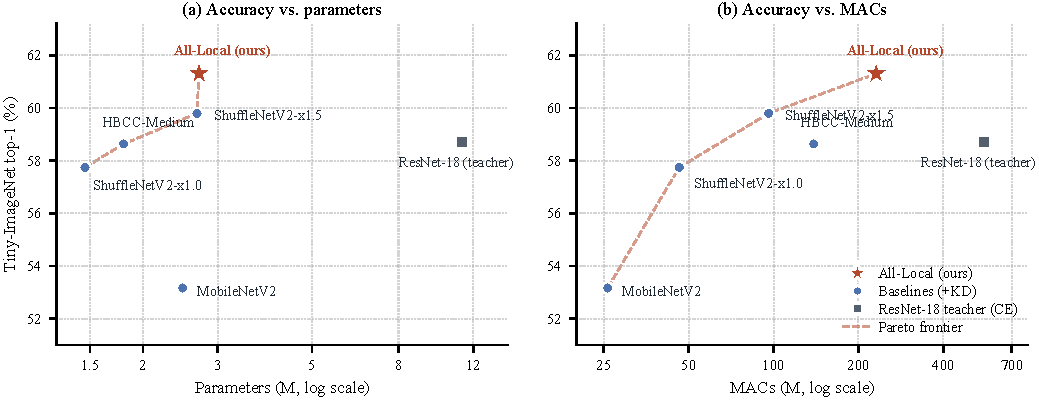
\includegraphics[width=\textwidth]{fig2_pareto.pdf}
\caption{Tiny-ImageNet accuracy against parameters (a) and against
multiply--accumulate operations (b), both on logarithmic axes. Accuracy is
the mean over three seeds; cost is measured on a Tesla T4 in a single
session. Every baseline shown is distilled from the same ResNet-18 teacher;
the teacher itself is trained with cross-entropy and is marked separately.
The proposed model lies on the parameter frontier but not on the operation
frontier.}
\label{fig:pareto}
\end{figure*}
